\documentclass[12pt]{article}

\usepackage{graphicx}
\usepackage{geometry}

\begin{document}

\newgeometry{left=1.5in,right=1in,top=1in,bottom=1.25in}
\linespread{1.5}

\begin{titlepage}
\center 
\textsc{\Large AUTOMATED GUIDED VEHICLE APPLICATION:}\\[1cm]
\textsc{\Large PRECISION AGRICULTURE}\\[6cm] 
\textsc{\Large Xiangnan Gong}\\[7cm] 
{\large Submitted to the faculty of the School of Informatics in partial fulfillment of the requirements for the degree of Master of Science in Electrical and Computer Engineering, Purdue University \\[0.5cm]Indianapolis, Indiana}\\[0.5cm] 
{\large \today}
\newpage
\pagestyle{empty}


\renewcommand{\contentsname}{Table of Contents}
\tableofcontents
\newpage
\listoftables

\newpage
\listoffigures

\newpage
\renewcommand{\abstractname}{\Large Abstruct}
\begin{abstract}
\normalsize
Nowadays, there are many types of automated guided vehicle (AGV) running in different field of industries. Typically their job is moving raw materials or parts around the manufacturing facility. And they can be very accurate in working by following the guide from the wires in the floor, magnets, laser, or vision. However, they all requires an indoor condition. Therefore, the purpose of this thesis report is to discuss the implement of the outdoor AGV. An outdoor AGV has much more constrains than indoor. The environment indoor can be easily controlled while the door is not. The condition could be rough ground, no preset guiding wire or magnets, vision blocking by dust, and so on. The solution, which will talk in this paper, to achieve the outdoor AGV is using laser or vision to guide. In addition, a buffer will be set to stabilize the cargo or others working devices, to prevent them from the shaking due to the rough ground. To be more specific, a prototype will be built to simulate the working of seeder. In agriculture, it is very important to plant corns in a straight line. It benefits not only in absorbing sunlight and ventilation, but also reduce the work of irrigation, fertilizing, and harvest. Because a straight line of corn also mean a straight line of aisle. And more importantly, to achieve unmanned agriculture, a corn field with straight line of aisle will be a good condition for other agriculture robots. 
\end{abstract}

\newpage
\end{titlepage}

\begin{flushleft}

\section{Introduction}

\subsection{Introduction to subject}
Introduce the idea of the design. Introduce the idea of the design. Introduce the idea of the design. Introduce the idea of the design. Introduce the idea of the design. Introduce the idea of the design. Introduce the idea of the design. Introduce the idea of the design. Introduce the idea of the design. Introduce the idea of the design. Introduce the idea of the design. Introduce the idea of the design. Introduce the idea of the design. Introduce the idea of the design. Introduce the idea of the design. Introduce the idea of the design. Introduce the idea of the design. Introduce the idea of the design. Introduce the idea of the design. Introduce the idea of the design. Introduce the idea of the design.\cite{bozer1991tandem}
AGV解放了很多劳动力,节省成本,提高效率。室内的做的很好,精准度很高(1 引用室内AGV)但是室外的略显不足。室外的环境条件复杂,地面不平,打滑,天气,铺设轨道不划算。本文将探讨一种新的设计方案,试图解决。
主要针对现在的农业育种实验田,以及将来的无人农场,所设计的,户外AGV。

\subsection{Importance of subject}
This is the Importance of subject. This is the Importance of subject. This is the Importance of subject. This is the Importance of subject. This is the Importance of subject. This is the Importance of subject. This is the Importance of subject. This is the Importance of subject. This is the Importance of subject. This is the Importance of subject. This is the Importance of subject. This is the Importance of subject. This is the Importance of subject. This is the Importance of subject. This is the Importance of subject. This is the Importance of subject. This is the Importance of subject. This is the Importance of subject. This is the Importance of subject. This is the Importance of subject. This is the Importance of subject. This is the Importance of subject. This is the Importance of subject. This is the Importance of subject. This is the Importance of subject. This is the Importance of subject. This is the Importance of subject. \cite{douglas2000navigation} \cite{egbelu1984characterization}
介绍重要性
就现在的农业育种试验田来说,播种的直非常重要
控制变量法,种的直可以有效地保证不同植株在相同的条件下生长(2 引用试验田需要条件)。光照,二氧化碳,肥料,水分。一切都已种的直为前提。
未来的无人农业,种的直则无人机器人更方便进入垄间工作(3 引用农业机器人),提高无人机器人的精准性,保护作物不被破坏。

\subsection{Knowledge gap}
This is the Knowledge gap.  This is the Knowledge gap. This is the Knowledge gap. This is the Knowledge gap. This is the Knowledge gap. This is the Knowledge gap. This is the Knowledge gap. 
\begin{figure}[h!]
	\begin{center}
		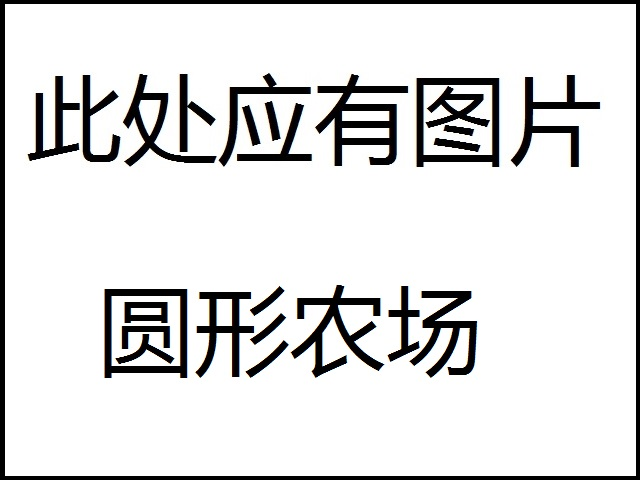
\includegraphics[scale = 0.6]{farm.jpg}
		\caption{Farm}
		%\label{figure 1}
	\end{center}
\end{figure}
This is the Knowledge gap. This is the Knowledge gap. This is the Knowledge gap. This is the Knowledge gap. This is the Knowledge gap. This is the Knowledge gap. This is the Knowledge gap. This is the Knowledge gap. This is the Knowledge gap. \cite{egbelu1986potentials}This is the Knowledge gap. This is the Knowledge gap. This is the Knowledge gap. This is the Knowledge gap. This is the Knowledge gap. This is the Knowledge gap. 
\begin{table}[h!]
	\begin{center}
		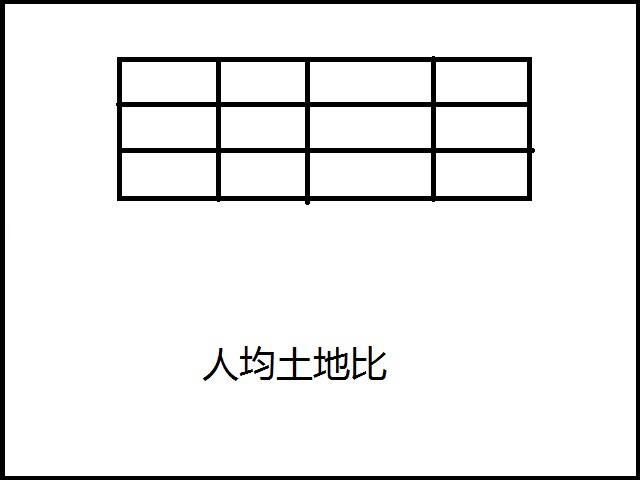
\includegraphics[scale = 0.6]{landratio.jpg}
		\caption{Landratio}
		%\label{table 1}
	\end{center}
\end{table}
This is the Knowledge gap. This is the Knowledge gap. This is the Knowledge gap. This is the Knowledge gap. This is the Knowledge gap. \cite{evers1996automated}This is the Knowledge gap. This is the Knowledge gap. This is the Knowledge gap. This is the Knowledge gap. This is the Knowledge gap. This is the Knowledge gap. This is the Knowledge gap. This is the Knowledge gap. This is the Knowledge gap. 
\begin{table}[h!]
	\begin{center}
		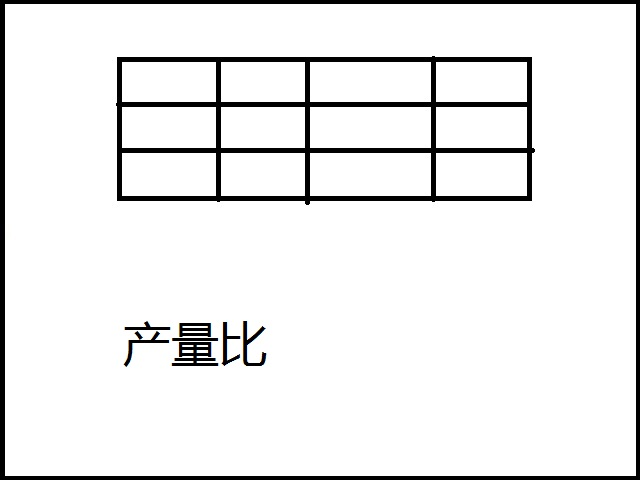
\includegraphics[scale = 0.6]{productivityratio.jpg}
		\caption{Productivityratio}
		%\label{table 1}
	\end{center}
\end{table}
This is the Knowledge gap. This is the Knowledge gap. This is the Knowledge gap. This is the Knowledge gap. This is the Knowledge gap. This is the Knowledge gap. This is the Knowledge gap. This is the Knowledge gap. This is the Knowledge gap.

This is the Knowledge gap. \cite{gaskins1987flow}


介绍传统农业和未来的无人农业的区别。美国的农业已经完善,形成了独有的农业形式,粗放型。地多,人少,资源多。土地浪费(4 引用大农场的圆形灌溉)(  图片农场俯视图),不是不能节约,而是现状成本低。但是像对于世界的其他地方,沙漠国家需要精准的滴管(5 引用滴灌),因为缺水。中国人多,人均地少(6 引用人均耕地),要更高效的利用土地,提高单位土地产量。(做图表 中美人均耕地比较,做图表,中国人均耕地和耕地产粮)发展未来精准农业不像在美国看起来那样不重要。

\section{Background}

\subsection{Related research}
This is the Related research. This is the Related research. This is the Related research. This is the Related research. This is the Related research. This is the Related research. This is the Related research. This is the Related research. This is the Related research. This is the Related research. This is the Related research. This is the Related research. This is the Related research. This is the Related research. This is the Related research. This is the Related research. This is the Related research. This is the Related research. This is the Related research. This is the Related research. This is the Related research. This is the Related research. \cite{lenain2006high}
列举现有的几种自动走直线农机(7 引用现有的农机),说明不足之处。

\subsection{Current understanding}
This is the Current understanding. This is the Current understanding. This is the Current understanding. \cite{lenain2006high}This is the Current understanding. This is the Current understanding. This is the Current understanding. This is the Current understanding. This is the Current understanding. This is the Current understanding. This is the Current understanding. This is the Current understanding. This is the Current understanding.\cite{douglas2000navigation} This is the Current understanding. This is the Current understanding. This is the Current understanding. This is the Current understanding. \cite{egbelu1984characterization}
现在普遍用的是GPS引导的人开农机,精确度不够,不能实现无人(7 引用现有农机的精准度)。
低精准也许符合现阶段要求,但是像育种这样的特殊需求不能满足(2),同时也不能满足未来的无人农业(3)。

\subsection{Hypothesis or research question}
This is the Hypothesis or research question. This is the Hypothesis or research question. This is the Hypothesis or research question. This is the Hypothesis or research question. This is the Hypothesis or research question. This is the Hypothesis or research question. This is the Hypothesis or research question. This is the Hypothesis or research question. This is the Hypothesis or research question. This is the Hypothesis or research question. This is the Hypothesis or research question. 
\begin{figure}[h!]
	\begin{center}
		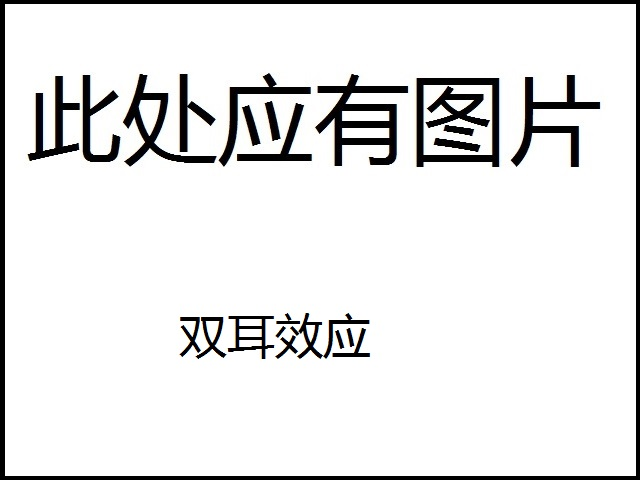
\includegraphics[scale = 0.6]{twoears.jpg}
		\caption{Twoears}
		%\label{figure 1}
	\end{center}
\end{figure}
This is the Hypothesis or research question. This is the Hypothesis or research question. This is the Hypothesis or research question. This is the Hypothesis or research question. This is the Hypothesis or research question. This is the Hypothesis or research question. This is the Hypothesis or research question. This is the Hypothesis or research question. This is the Hypothesis or research question. This is the Hypothesis or research question. This is the Hypothesis or research question. This is the Hypothesis or research question. This is the Hypothesis or research question. This is the Hypothesis or research question. This is the Hypothesis or research question. This is the Hypothesis or research question. This is the Hypothesis or research question. This is the Hypothesis or research question. This is the Hypothesis or research question. This is the Hypothesis or research question. This is the Hypothesis or research question. This is the Hypothesis or research question. This is the Hypothesis or research question. This is the Hypothesis or research question. This is the Hypothesis or research question. This is the Hypothesis or research question. This is the Hypothesis or research question. This is the Hypothesis or research question. This is the Hypothesis or research question. This is the Hypothesis or research question. This is the Hypothesis or research question. This is the Hypothesis or research question. This is the Hypothesis or research question. This is the Hypothesis or research question. This is the Hypothesis or research question. This is the Hypothesis or research question. This is the Hypothesis or research question. This is the Hypothesis or research question. This is the Hypothesis or research question. This is the Hypothesis or research question. This is the Hypothesis or research question. This is the Hypothesis or research question. This is the Hypothesis or research question. This is the Hypothesis or research question. 
\begin{figure}[h!]
	\begin{center}
		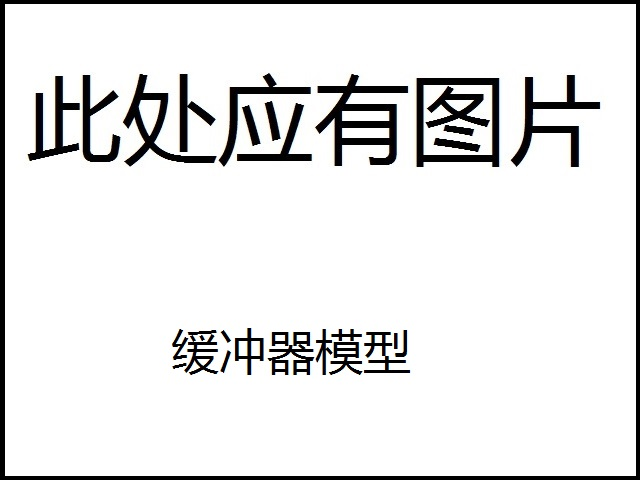
\includegraphics[scale = 0.6]{buffer.jpg}
		\caption{Buffer}
		%\label{figure 1}
	\end{center}
\end{figure}
This is the Hypothesis or research question. This is the Hypothesis or research question. This is the Hypothesis or research question. This is the Hypothesis or research question. This is the Hypothesis or research question. This is the Hypothesis or research question. This is the Hypothesis or research question.\cite{bozer1991tandem} 
如何能实现直线播种。借鉴室内AGV非常精准的解决方法(1),综合考虑拟人仿生.视觉(和听觉,双耳效应,引用,做图片说明)是最好的解决方案。第一步,激光引导,第二步,参照物引导,第三步,无引导,纯靠看到的图像自动选择参照物引导。
激光引导分为1D 2D 3D引导。 1D左右移动,摄像头看点,2D加入前后移动,3D加入旋转,摄像头看线段。(做图片说明)

\subsection{Intended project}
This is the Intended project. This is the Intended project. This is the Intended project. This is the Intended project. This is the Intended project. This is the Intended project. This is the Intended project. This is the Intended project. This is the Intended project. This is the Intended project. This is the Intended project. This is the Intended project. This is the Intended project. This is the Intended project. This is the Intended project. This is the Intended project. This is the Intended project. This is the Intended project. This is the Intended project. This is the Intended project. This is the Intended project. This is the Intended project. This is the Intended project. This is the Intended project. This is the Intended project. This is the Intended project. This is the Intended project. This is the Intended project. This is the Intended project. This is the Intended project. This is the Intended project. This is the Intended project. This is the Intended project. This is the Intended project. This is the Intended project. This is the Intended project. This is the Intended project. This is the Intended project. This is the Intended project. This is the Intended project. This is the Intended project. This is the Intended project. This is the Intended project. This is the Intended project. This is the Intended project. This is the Intended project. This is the Intended project. This is the Intended project. This is the Intended project. This is the Intended project. This is the Intended project. This is the Intended project. This is the Intended project. This is the Intended project. This is the Intended project. This is the Intended project. This is the Intended project. This is the Intended project. This is the Intended project. This is the Intended project. This is the Intended project. This is the Intended project. This is the Intended project. This is the Intended project. This is the Intended project. This is the Intended project. This is the Intended project. This is the Intended project. This is the Intended project. This is the Intended project. 
为实现第一步,在现有农机上进行改装,增加缓冲装置(特点),以提高精确度。制作模型进行试验。使用树莓派来对摄像头采集的图像进行处理,从而引导农机走直线。同时利用步进马达进行微调整,应付突发情况和误差。比如突然被石头搬到,突然打滑,农机突然偏离路径,无法马上回归,此时用带有步进马达的缓冲装置进行补救。而且农机很大,进行厘米级的移动困难而且耗费时间,有了缓冲装置可以减少很多误差。

\section{Methods}

\subsection{Materials and instruments}
This is the Materials and instruments. This is the Materials and instruments. This is the Materials and instruments. This is the Materials and instruments. This is the Materials and instruments. This is the Materials and instruments. This is the Materials and instruments. This is the Materials and instruments. This is the Materials and instruments. This is the Materials and instruments. This is the Materials and instruments. This is the Materials and instruments. This is the Materials and instruments. This is the Materials and instruments. 
\begin{table}[h!]
	\begin{center}
		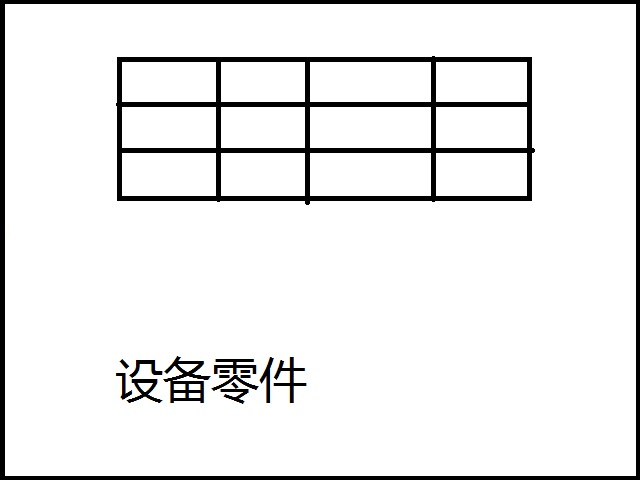
\includegraphics[scale = 0.6]{parts.jpg}
		\caption{Parts}
		%\label{table 1}
	\end{center}
\end{table}
This is the Materials and instruments. This is the Materials and instruments. This is the Materials and instruments. This is the Materials and instruments. This is the Materials and instruments. This is the Materials and instruments. 
对现有农机进行改装,所以成本低。现在实验阶段使用的是,电源,树莓派,摄像头,步进马达,框架,幕布,激光。(做图表,列出成本)

\subsection{Laser guided}

\subsubsection{Imaging processing}
This is the Animal or human subject clearance. This is the Animal or human subject clearance. This is the Animal or human subject clearance. This is the Animal or human subject clearance. This is the Animal or human subject clearance. This is the Animal or human subject clearance. This is the Animal or human subject clearance. This is the Animal or human subject clearance. This is the Animal or human subject clearance. This is the Animal or human subject clearance. This is the Animal or human subject clearance. This is the Animal or human subject clearance. 
\begin{figure}[h!]
	\begin{center}
		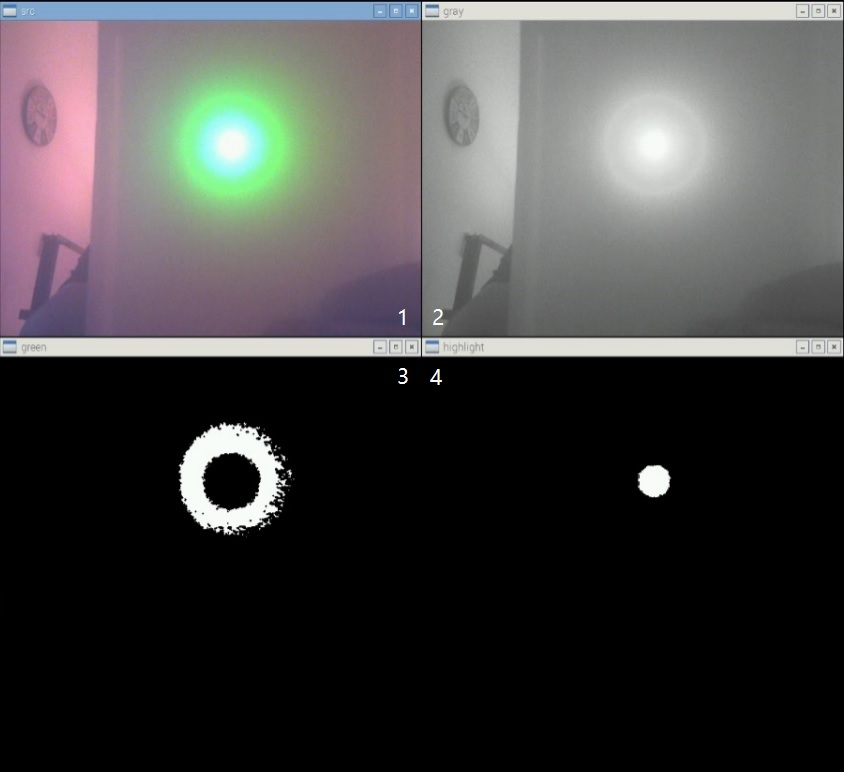
\includegraphics[scale = 0.6]{imaging.jpg}
		\caption{Imaging}
		%\label{figure 1}
	\end{center}
\end{figure}
This is the Animal or human subject clearance. This is the Animal or human subject clearance. This is the Animal or human subject clearance. This is the Animal or human subject clearance. This is the Animal or human subject clearance. This is the Animal or human subject clearance. This is the Animal or human subject clearance. This is the Animal or human subject clearance. This is the Animal or human subject clearance. This is the Animal or human subject clearance. This is the Animal or human subject clearance. This is the Animal or human subject clearance. This is the Animal or human subject clearance. This is the Animal or human subject clearance. 
用摄像头采集幕布上的光斑( 做图片,截图),分析其位置( 算法和公式),做出反馈。 给农机信号,使其左右转弯来保持直线轨迹。同时给缓冲器信号,使播种设备保持位置。

\subsubsection{Buffer design}
This is the buffer design. This is the buffer design. This is the buffer design. This is the buffer design. This is the buffer design. This is the buffer design. This is the buffer design. This is the buffer design. This is the buffer design. 
\begin{figure}[h!]
	\begin{center}
		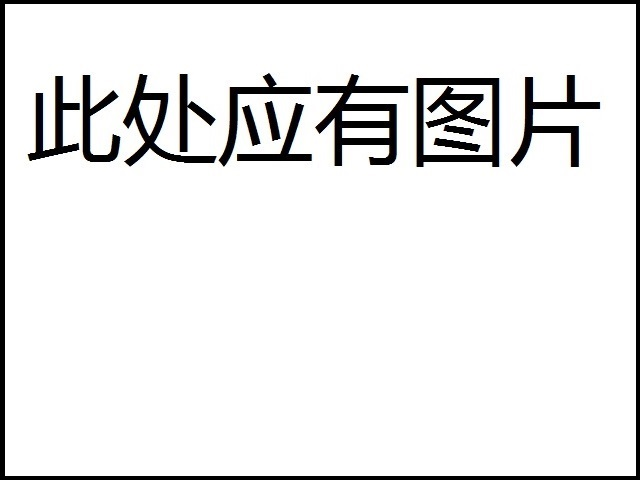
\includegraphics[scale = 0.6]{1D.jpg}
		\caption{1D}
		%\label{figure 1}
	\end{center}
\end{figure}
This is the buffer design. This is the buffer design. This is the buffer design. This is the buffer design. This is the buffer design. This is the buffer design. This is the buffer design. This is the buffer design. This is the buffer design. 
\begin{figure}[h!]
	\begin{center}
		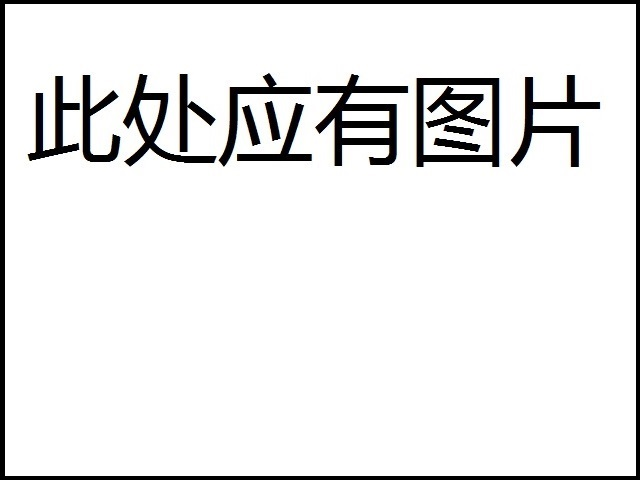
\includegraphics[scale = 0.6]{2D.jpg}
		\caption{2D}
		%\label{figure 1}
	\end{center}
\end{figure}
This is the buffer design. This is the buffer design. This is the buffer design. This is the buffer design. This is the buffer design. This is the buffer design. This is the buffer design. This is the buffer design. This is the buffer design. This is the buffer design. 
步进马达接收信号,在轨道上带着摄像头和播种设备移动。(做图片)首先实现1D移动,(做图片)再实现2D移动。

\subsubsection{Improvement}
This is the improvement. This is the improvement. This is the improvement. This is the improvement. This is the improvement. This is the improvement. This is the improvement. This is the improvement. This is the improvement. This is the improvement. 
\begin{figure}[h!]
	\begin{center}
		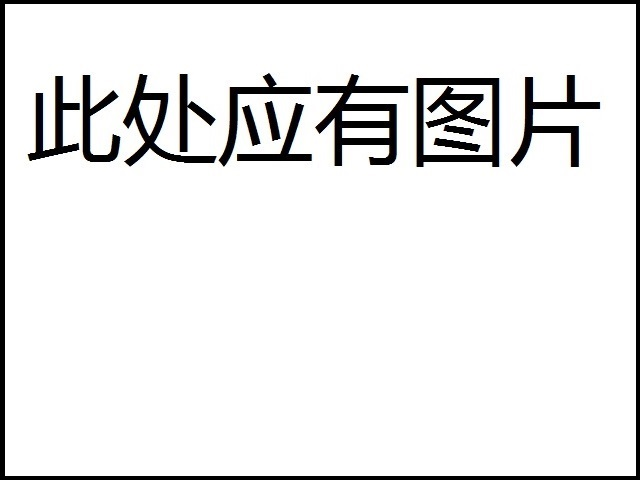
\includegraphics[scale = 0.6]{3D.jpg}
		\caption{3D}
		%\label{figure 1}
	\end{center}
\end{figure}
This is the improvement. This is the improvement. This is the improvement. This is the improvement. This is the improvement. This is the improvement. This is the improvement. This is the improvement. This is the improvement. This is the improvement. This is the improvement. This is the improvement. This is the improvement. 
\begin{figure}[h!]
	\begin{center}
		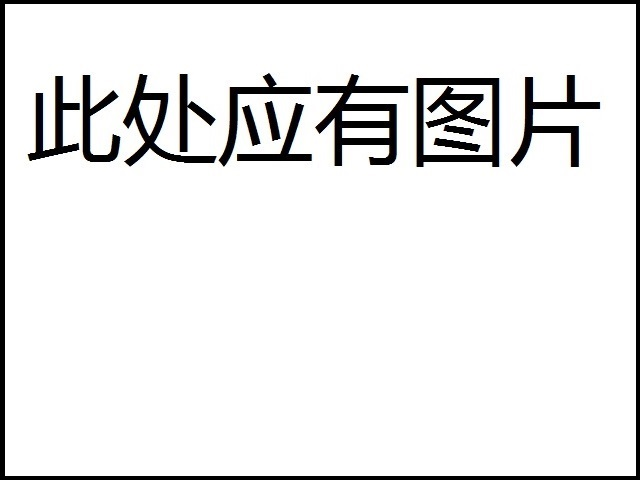
\includegraphics[scale = 0.6]{curtain.jpg}
		\caption{Curtain}
		%\label{figure 1}
	\end{center}
\end{figure}
This is the improvement. This is the improvement. This is the improvement. This is the improvement. 
为实现3D移动,摄像头需要旋转( 做图片CAD),幕布需要特制,要能显示激光的线段而不是点( 做图片CAD)。图像处理的算法和公式。

\subsection{Object guided}
This is the object guided. This is the object guided. This is the object guided. This is the object guided. This is the object guided. This is the object guided. This is the object guided. This is the object guided. This is the object guided. This is the object guided. This is the object guided. This is the object guided. This is the object guided. This is the object guided. This is the object guided. This is the object guided. This is the object guided. 
\begin{figure}[h!]
	\begin{center}
		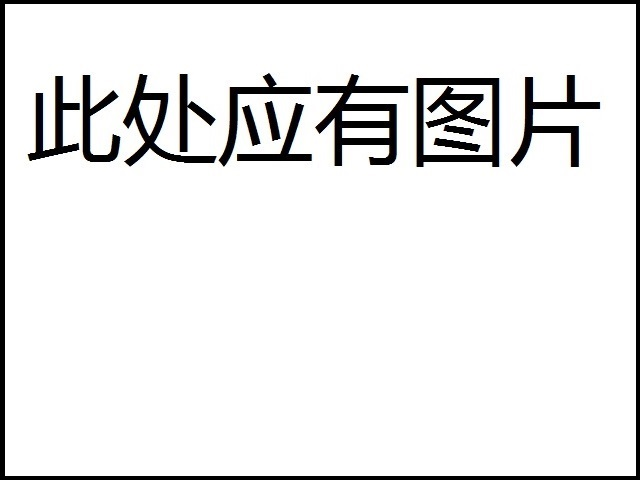
\includegraphics[scale = 0.6]{objectperspective.jpg}
		\caption{Objectperspective}
		%\label{figure 1}
	\end{center}
\end{figure}
This is the object guided. This is the object guided. This is the object guided. This is the object guided. This is the object guided. This is the object guided. This is the object guided. This is the object guided. This is the object guided. This is the object guided. 
在田边放置鲜明物体,例如交通锥Traffic Cone,通过摄像头识别该物体进行导航。少许透视算法,保持物体在屏幕中间好算,公式 ( 做图片)

\subsection{Vision guided}
This is the vision guided. This is the vision guided. This is the vision guided. This is the vision guided. This is the vision guided. This is the vision guided. This is the vision guided. This is the vision guided. This is the vision guided. This is the vision guided. This is the vision guided. This is the vision guided. This is the vision guided. This is the vision guided. This is the vision guided. This is the vision guided. This is the vision guided. This is the vision guided. This is the vision guided. This is the vision guided. This is the vision guided. This is the vision guided. This is the vision guided. This is the vision guided. This is the vision guided. This is the vision guided. This is the vision guided. This is the vision guided. This is the vision guided. This is the vision guided. This is the vision guided. This is the vision guided. This is the vision guided. 
\begin{figure}[h!]
	\begin{center}
		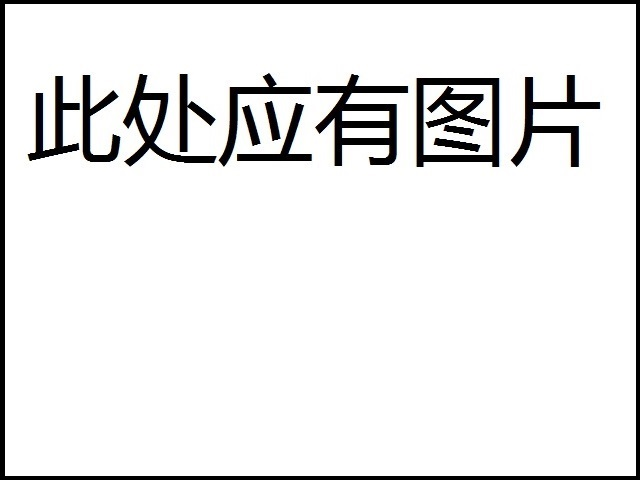
\includegraphics[scale = 0.6]{perspective.jpg}
		\caption{Perspective}
		%\label{figure 1}
	\end{center}
\end{figure}
This is the vision guided. This is the vision guided. This is the vision guided. This is the vision guided. 
不使用特殊物体,程序自动选择一个易识别物体来进行导航,例如树的树干,地平线。物体不在屏幕中间,高级透视算法,公式,(做图片)

\subsection{Alternate plans: Ultrasonic guided}
This is the Alternate plans. This is the Alternate plans. This is the Alternate plans. This is the Alternate plans. This is the Alternate plans. This is the Alternate plans. This is the Alternate plans. This is the Alternate plans. This is the Alternate plans. This is the Alternate plans. This is the Alternate plans. This is the Alternate plans. This is the Alternate plans. This is the Alternate plans. This is the Alternate plans. This is the Alternate plans. This is the Alternate plans. This is the Alternate plans. This is the Alternate plans. This is the Alternate plans. This is the Alternate plans. This is the Alternate plans. This is the Alternate plans. 
\begin{figure}[h!]
	\begin{center}
		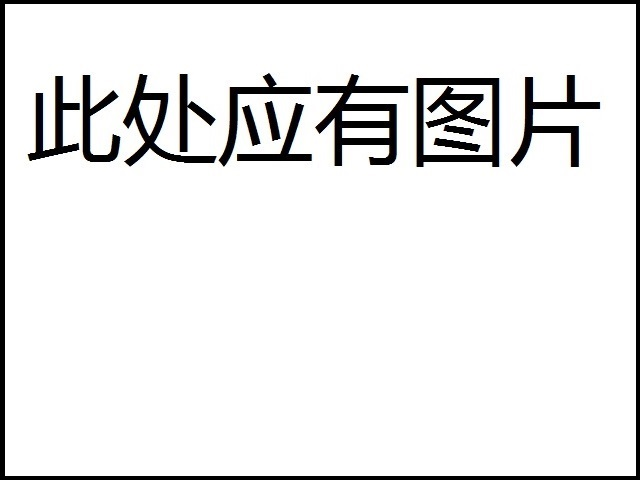
\includegraphics[scale = 0.6]{twoearsdesign.jpg}
		\caption{Twoearsdesign}
		%\label{figure 1}
	\end{center}
\end{figure}
This is the Alternate plans. This is the Alternate plans. This is the Alternate plans. This is the Alternate plans.\cite{muller1983automated} This is the Alternate plans. This is the Alternate plans. This is the Alternate plans. This is the Alternate plans. 
利用双耳效应(8引用),一个超声波源,两个接收器。生源要有特殊性,不容易被干扰,好识别。算法,公式,(做图片)

\section{Results}

\subsection{Introduction}
This is the Introduction. This is the Introduction. This is the Introduction. This is the Introduction. This is the Introduction. This is the Introduction. This is the Introduction. This is the Introduction. This is the Introduction. This is the Introduction. This is the Introduction. This is the Introduction. This is the Introduction. This is the Introduction. This is the Introduction. This is the Introduction. This is the Introduction. This is the Introduction. This is the Introduction. This is the Introduction. This is the Introduction. This is the Introduction. This is the Introduction. This is the Introduction. This is the Introduction. This is the Introduction. This is the Introduction. This is the Introduction. 
使用这个设备能达到那些效果。
,为农业育种提供方便,为未来的无人农业提供先决条件。

\subsection{Important highlights}
This is the Important highlights. This is the Important highlights. This is the Important highlights. This is the Important highlights. This is the Important highlights. This is the Important highlights. This is the Important highlights. This is the Important highlights. This is the Important highlights. This is the Important highlights. This is the Important highlights. This is the Important highlights. This is the Important highlights. This is the Important highlights. This is the Important highlights. This is the Important highlights. This is the Important highlights. This is the Important highlights. This is the Important highlights. This is the Important highlights. This is the Important highlights. This is the Important highlights. This is the Important highlights. This is the Important highlights. This is the Important highlights. This is the Important highlights. This is the Important highlights. This is the Important highlights. This is the Important highlights. 
利用摄像头来引导是趋势,摄像头成本低,易于改进,人就是靠视觉获取信息,同样机器也可以

\subsection{Feasibility}
This is the feasibility. This is the feasibility. This is the feasibility. This is the feasibility. This is the feasibility. This is the feasibility. This is the feasibility. This is the feasibility. This is the feasibility. This is the feasibility. This is the feasibility. This is the feasibility. This is the feasibility. This is the feasibility. This is the feasibility. This is the feasibility. This is the feasibility. This is the feasibility. This is the feasibility. This is the feasibility. This is the feasibility. This is the feasibility. This is the feasibility. This is the feasibility. This is the feasibility. This is the feasibility. This is the feasibility. This is the feasibility. This is the feasibility. This is the feasibility. This is the feasibility. This is the feasibility. This is the feasibility. This is the feasibility. This is the feasibility. This is the feasibility. This is the feasibility. This is the feasibility. This is the feasibility. This is the feasibility. This is the feasibility. \cite{vis2006survey}This is the feasibility. This is the feasibility. This is the feasibility. This is the feasibility. 
现在中国的农业育种试验田非常需要。(9 引用)中国农业落后,雇佣农民成本在增加,而且他们不懂,不理解种的直的重要性。由于是在现有农机上改装,无论多落后的农机都可以。成本不高。效率高。花很少的钱能提高很多精准度。对于未来农业也很有必要。

\subsection{Constraints}
This is the constraints. This is the constraints. This is the constraints. This is the constraints. This is the constraints. This is the constraints. This is the constraints. This is the constraints. This is the constraints. This is the constraints. This is the constraints. This is the constraints. This is the constraints. This is the constraints. This is the constraints. This is the constraints. This is the constraints. This is the constraints. This is the constraints. This is the constraints. This is the constraints. This is the constraints. This is the constraints. This is the constraints. This is the constraints. This is the constraints. This is the constraints. This is the constraints. This is the constraints. This is the constraints. This is the constraints. This is the constraints. This is the constraints. This is the constraints. This is the constraints. This is the constraints. This is the constraints. \cite{vis2006survey} This is the constraints. This is the constraints. This is the constraints. This is the constraints. 
激光,物体,纯视觉,都基于摄像头,所以摄像头的限制就是这个设备的限制。比如光线强弱,扬尘遮挡,下雨。对于激光来说,激光的角度不太好定位,射程,功率,国标限制,不当操作对人的危害(9引用)。声音来说,声音的强度和干扰。增加声音设备,成本增加。

\subsection{Application to other areas}
This is the application to other areas. This is the application to other areas. This is the application to other areas. This is the application to other areas. This is the application to other areas. This is the application to other areas. This is the application to other areas. This is the application to other areas. This is the application to other areas. This is the application to other areas. This is the application to other areas. This is the application to other areas. This is the application to other areas. This is the application to other areas. This is the application to other areas. This is the application to other areas. This is the application to other areas. This is the application to other areas. This is the application to other areas. This is the application to other areas. This is the application to other areas. This is the application to other areas. 
不只是农业可以使用户外AGV,其他户外工作也能使用。比如修路,建筑,伐木。

\section{Conclusion}

\subsection{Importance of outdoor-AGV}
This is the importance of outdoor-AGV. This is the importance of outdoor-AGV. This is the importance of outdoor-AGV. This is the importance of outdoor-AGV. This is the importance of outdoor-AGV. This is the importance of outdoor-AGV. This is the importance of outdoor-AGV. This is the importance of outdoor-AGV. This is the importance of outdoor-AGV. This is the importance of outdoor-AGV. This is the importance of outdoor-AGV. This is the importance of outdoor-AGV. This is the importance of outdoor-AGV. This is the importance of outdoor-AGV. This is the importance of outdoor-AGV. This is the importance of outdoor-AGV. This is the importance of outdoor-AGV. This is the importance of outdoor-AGV. This is the importance of outdoor-AGV. This is the importance of outdoor-AGV. This is the importance of outdoor-AGV. This is the importance of outdoor-AGV. This is the importance of outdoor-AGV. This is the importance of outdoor-AGV. This is the importance of outdoor-AGV. This is the importance of outdoor-AGV. This is the importance of outdoor-AGV. This is the importance of outdoor-AGV. This is the importance of outdoor-AGV. This is the importance of outdoor-AGV. This is the importance of outdoor-AGV. 
本文重点讨论了关于户外AGV在农业方面的应用,现在工厂有流水线,但是室外的农业却没有这么高效率。目前来说,传统的GPS农机或许在播种上能满足现在的需求。但是要满足育种试验田的播种需求,还是需要户外AGV。放眼未来,要实现想工厂流水线一样高效的无人农业,精准的播种是第一步也是非常重要的一步。

\subsection{Overview of significants}
This is the Overview of significant findings. This is the Overview of significant findings. This is the Overview of significant findings. This is the Overview of significant findings. This is the Overview of significant findings. This is the Overview of significant findings. This is the Overview of significant findings. This is the Overview of significant findings. This is the Overview of significant findings. This is the Overview of significant findings. This is the Overview of significant findings. This is the Overview of significant findings. This is the Overview of significant findings. This is the Overview of significant findings. This is the Overview of significant findings. This is the Overview of significant findings. This is the Overview of significant findings. This is the Overview of significant findings. This is the Overview of significant findings. This is the Overview of significant findings. 
本文讨论了多种播种机器人的实现方式。使用激光简单易行,1D 2D 3D,使用物体更方便,不需要校准激光,使用视觉是最终目的,最终实现完全无人
精准度提高,因为改装,所以容易实现,实现成本低

\subsection{Limitations}
This is the limitations. This is the limitations. This is the limitations. This is the limitations. This is the limitations. This is the limitations. This is the limitations. This is the limitations. This is the limitations. This is the limitations. This is the limitations. This is the limitations. This is the limitations. This is the limitations. This is the limitations. This is the limitations. This is the limitations. This is the limitations. This is the limitations. This is the limitations. This is the limitations. This is the limitations. This is the limitations. This is the limitations. This is the limitations. This is the limitations. This is the limitations. This is the limitations. This is the limitations. This is the limitations. This is the limitations. This is the limitations. This is the limitations. This is the limitations. This is the limitations. This is the limitations. This is the limitations. This is the limitations. This is the limitations. This is the limitations. This is the limitations. 
美国农业粗放,地多,资源多,不需要这么精打细算。但是世界上的其他地区还是需要的,无人机的精准农业能带来可观的效益。虽然现在技术上不完善,但无人农业是大趋势。这个户外AGV也可以应用的很多其他的领域。

\subsection{Further improvement}
This is the Recommendations for further research. This is the Recommendations for further research. This is the Recommendations for further research. This is the Recommendations for further research. This is the Recommendations for further research. This is the Recommendations for further research. This is the Recommendations for further research. This is the Recommendations for further research. This is the Recommendations for further research. This is the Recommendations for further research. This is the Recommendations for further research. This is the Recommendations for further research. This is the Recommendations for further research. This is the Recommendations for further research. This is the Recommendations for further research. This is the Recommendations for further research. This is the Recommendations for further research. This is the Recommendations for further research. This is the Recommendations for further research. \cite{wu2004modeling}
圆形轨迹,适应不同地形,如山地,梯田。不只是播种,可以浇水施肥撒药,采摘水果,看颜色,熟的摘。实现无人农业。



\newpage
\section{REFERENCES}
\bibliographystyle{apalike}
\bibliography{bibfile}

\newpage
\appendix
\renewcommand{\appendixname}{Appendix~\Alph{section}}

\section{Appendix A}
This is appendix A

\end{flushleft}
\end{document}
